\chapter{Towards Tunable Laser with On-Chip Controllable Feedback}\label{ch:Towards_laser_with_on_chip_controllable_feedback}
In this chapter, design of hybrid polymer-based tunable laser with on-chip controllable feedback is presented by combining the Polyboard technology \cite{zhang2011polymer} with InP components. Two seperate designs are presented, one is focusd on bandwidth enhancement by photon-photon resonance and the other is linewidth reduction. The elements used for the design and the first characterization of the produced photonic integrated circuits (PICs) are presented.

\section{Design and Characterization}\label{sec:design_and_characterization}
The design of the on-chip controllable feedback is targeting to the weak feedback region with phase dependent linewidth reduction and strong feedback region with coumpound cavity mode \cite{petermann2012laser,ohtsubo2012semiconductor}. Elements involved including the Bragg grating, Multimode Interferometer (MMI), Variable Optical Attenuator (VOA) and Thin Film Filter (TFF) structures on the Polyboard platform. Design principle and the characterization of the devices are shown in the following sections.
% \begin{figure}[ht]
%     \centering
%     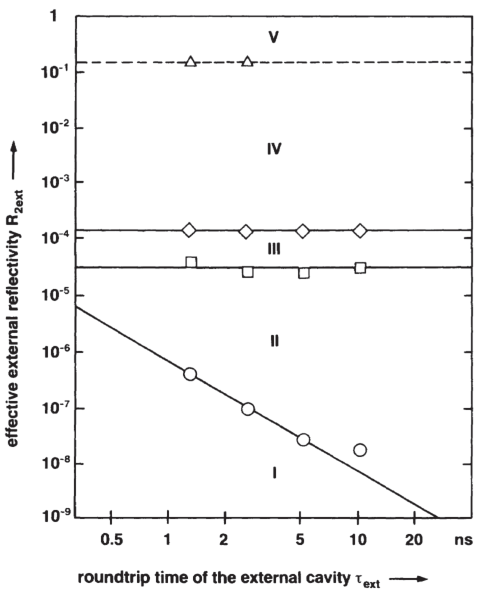
\includegraphics[width=10cm]{figures/feedback_region.PNG}
%     \caption{Feedback regimes for a laser diode.}
%     \label{feedback_region}
% \end{figure}


% \subsection{Passive Elements}
% As a variable optical attenuator (VOA) a 1x1 thermally tunable Multimode interferometer (MMI) is used (Fig.3.4.c). MMI is a multimode waveguide in which the light propagates in N modes. The various modes interfere with each other and produce an interference pattern in the MMI. This pattern allows at points of constructive interference to place output waveguide and thus to tap multiple outputs, each with a corresponding proportion of the total output power from an input signal. Depending on the design of the structure, the MMI can realize a different power division. On one side along the MMI is placed an electrode that allows using the thermo-optical effect. 
% We distinguish the states ON and OFF. In the OFF state, there is no heating of the electrodes and constructive interference takes place at the point where the output waveguide is. In ON-state, the interference pattern of the MMI is so affected, so that shifts through the partial change of the refractive index of the MMI, the position of constructive interference. Thus, a maximum interference point moves away from the position of the output waveguide and the output signal is tapped at reduced power (Fig.3.4.a and b). In this way a variable optical attenuation is created.
% An input waveguide with a width and height of 3.2 µm leads light into the interferometer. The height of the MMI (x-axis) also corresponds to 3.2 µm, the width is 18 µm and the length is 380 µm. The light that is leaving the MMI is received by an output waveguide. Height and width of the output waveguide coincide with the dimensions of the input waveguide. The transition of the input and output waveguide of the MMI is realized with taper sections that reduce the coupling losses. This VOA design was showing the best results compare to the literature [16-18].


% The Multimode Interferometer (MMI) is a multimode waveguide in which the light propagates in N modes. The various modes interfere with each other and produce an interference pattern in the MMI. This pattern allows at points of constructive interference to place output waveguide and thus to tap multiple outputs, each with a corresponding proportion of the total output power from an input signal. Depending on the design of the structure, the MMI can realize a different power division.



\subsection{Short Feedback Cavity} \label{subsec:short_feedback_cavity}
The on-chip short feedback cavity design is shown in \autoref{fig:grating_6559}, it is achieved by an additional waveguide and a TFF slot after the normal tunable DBR laser, followed by a $1\times 2$ MMI to seperate the output port and the external cavity. In the external cavity, VOA and phase section are included. The grating is designed to have its Bragg wavelength at $\lambda_B=1550 \ nm$.  Variable Optical Attenuator (VOA) is acheived with a $1\times 1$  thermally tunable MMI by placing an electrode on the side along the MMI which allows the thermo-optical effect. Thin Film Filter (TFF) acts as a high reflectivity mirror with its operating wavelength covers the grating Bragg wavelength, it can be simply inserted in the TFF slot thanks to the Polyboard technology. 

\begin{figure}[H]
    \centering
    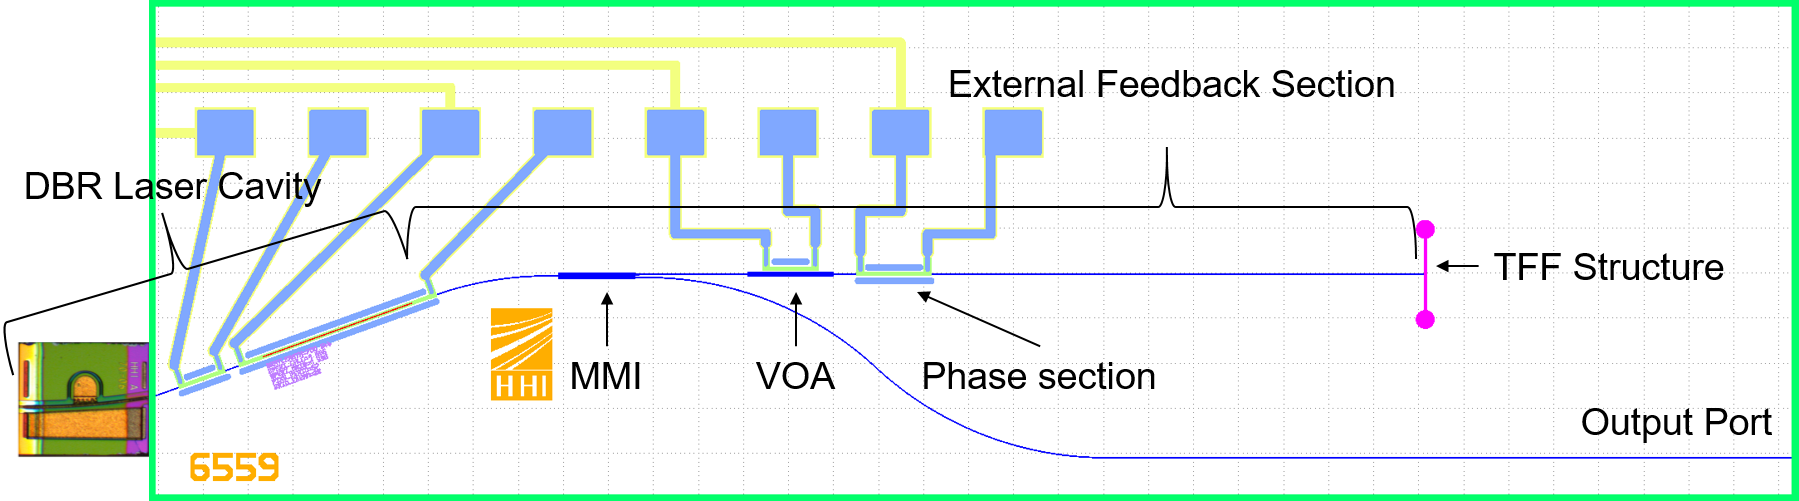
\includegraphics[width=\linewidth]{figures/6559_short_comment.png}
    \caption{Chip design of the laser with a short external section and controllable feedback.}
    \label{fig:grating_6559_design}
\end{figure}

In order to exploit PPR, \autoref{eq:mode_spacing_FSR} is used to set the ideal cavity length in combine with \autoref{tab:PPR_FSR} as shown below. External cavity length of [3129.76, 3589,76, 3859.76, 4159.76, 4869.76, 5309.76, 6359.76] $\mu m$ are choosen according to the calculated FSR plot shown in \autoref{fig:design_FSR}.

\begin{table}[ht]
    \centering
    \caption{Parameters used for the calculation for PPR in the short feedback design.}
    \label{tab:PPR_FSR}
    \begin{tabular}{@{}lll@{}}
    \toprule
    Symbol          & Description                      & Value             \\ \midrule
    $L_{gain}$      & Active section length            & $300 \ \mu m$     \\
    $L_{phase}$     & Phase section length             & $525 \ \mu m$     \\
    $L_{grating}$   & Grating section length           & $700 \ \mu m$     \\
    $n_{gain}$      & Active section refractive index  & 3.2               \\
    $n_{poly}$      & Polymer refractive index         & 1.46              \\
    \bottomrule
    \end{tabular}
\end{table}

\begin{figure}[H]
    \centering
    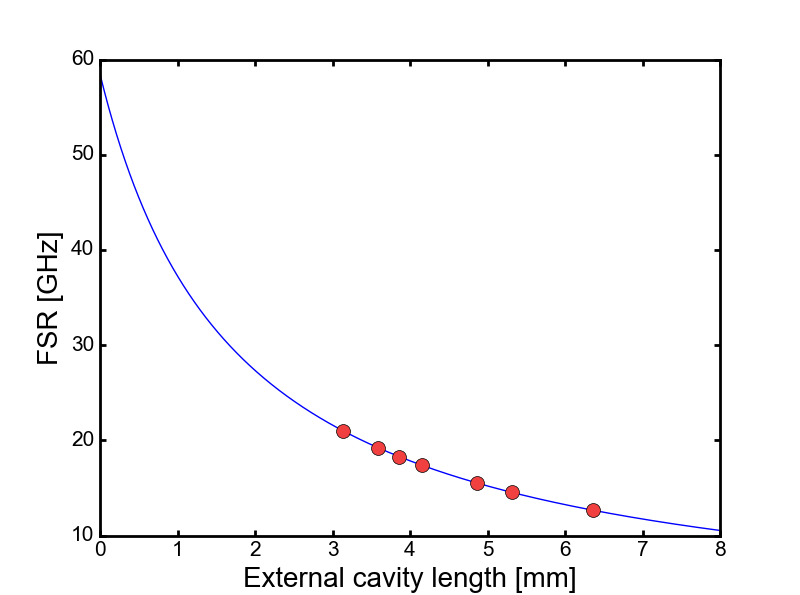
\includegraphics[width=.7\linewidth]{figures/design_FSR.png}
    \caption{FSR versus different external cavity length, the red circle markers are corresponding to the FSR of [21.7, 19.8, 18.8, 17.8, 15.9, 14.9, 12.9] $GHz$.}
    \label{fig:design_FSR}
\end{figure}

The example of produced photonic integrated circuits (PICs) and grating characterization is shown in \autoref{fig:grating_6559}. The appearing of the ripples in the transmission and reflection curves indicates the existing of the strong reflection along with the grating. The calculated mode spacing is corresponding to the external feedback section and the distance between the MMI and the output port respectively, which indicates the reflection from the TFF slot is relatively high in this case. The characterization example of the VOA is shown in \autoref{fig:VOA_18321}. Maximum $-28.39 \ dB$ damping was achieved at current value of $54 \ mA$. 

\begin{figure}[H]
    \centering
    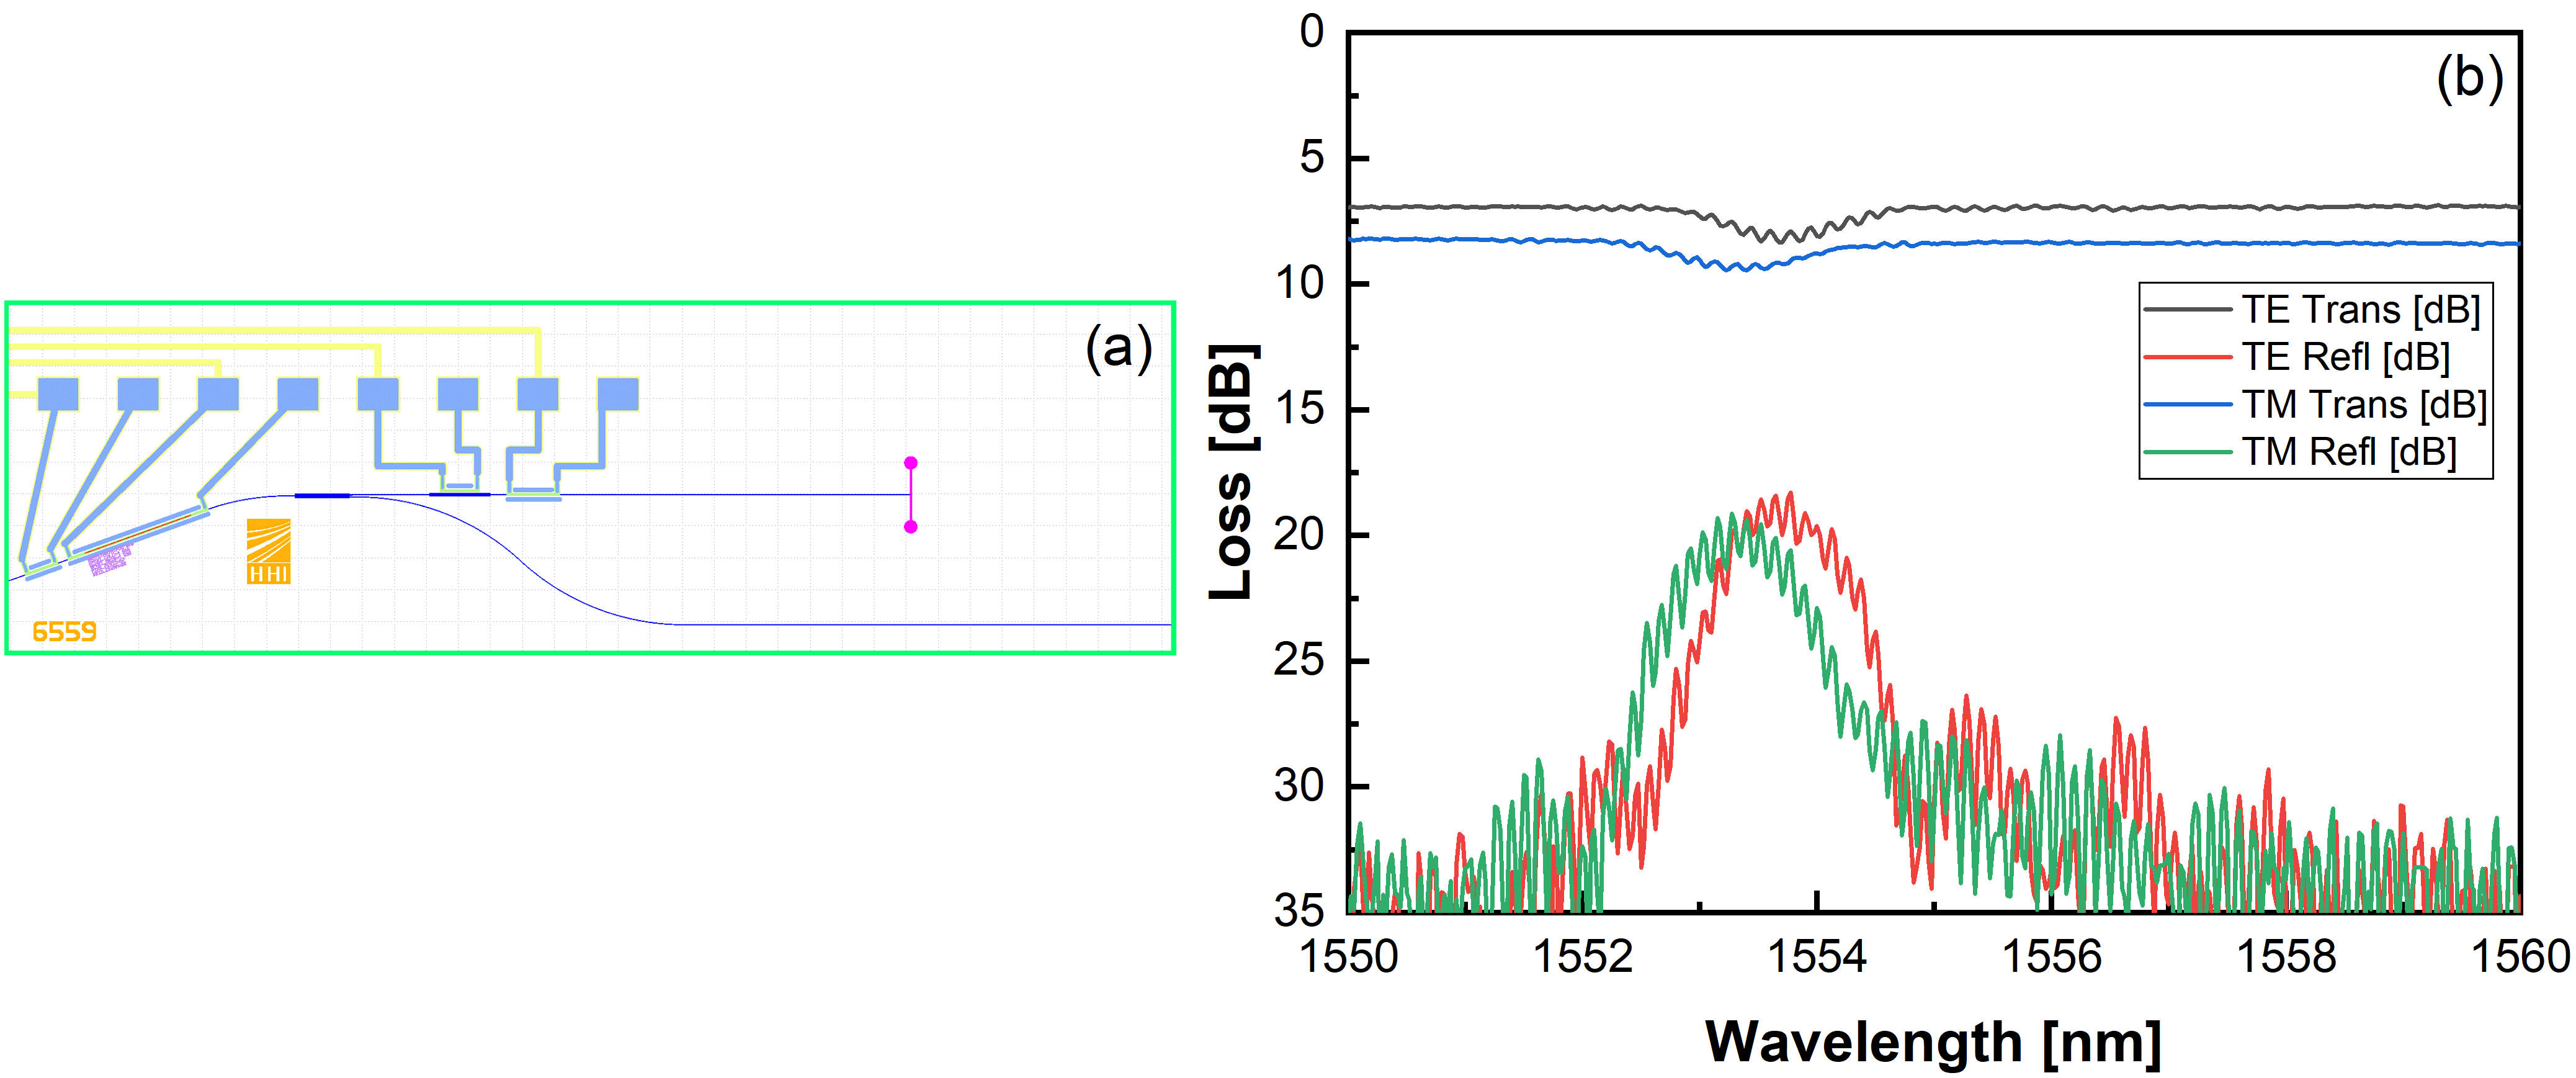
\includegraphics[width=\linewidth]{figures/grating_6559.png}
    \caption{(a) Produced photonic integrated circuits (PICs) with short feedback design, (b)grating characterization of the device, the spacing of the ripples in the transmission (black and blue) and reflection (red and green) curves are corresponding to the length of the external cavity and the distance between MMI and output port respectively.}
    \label{fig:grating_6559}
\end{figure}

\begin{figure}[H]
    \centering
    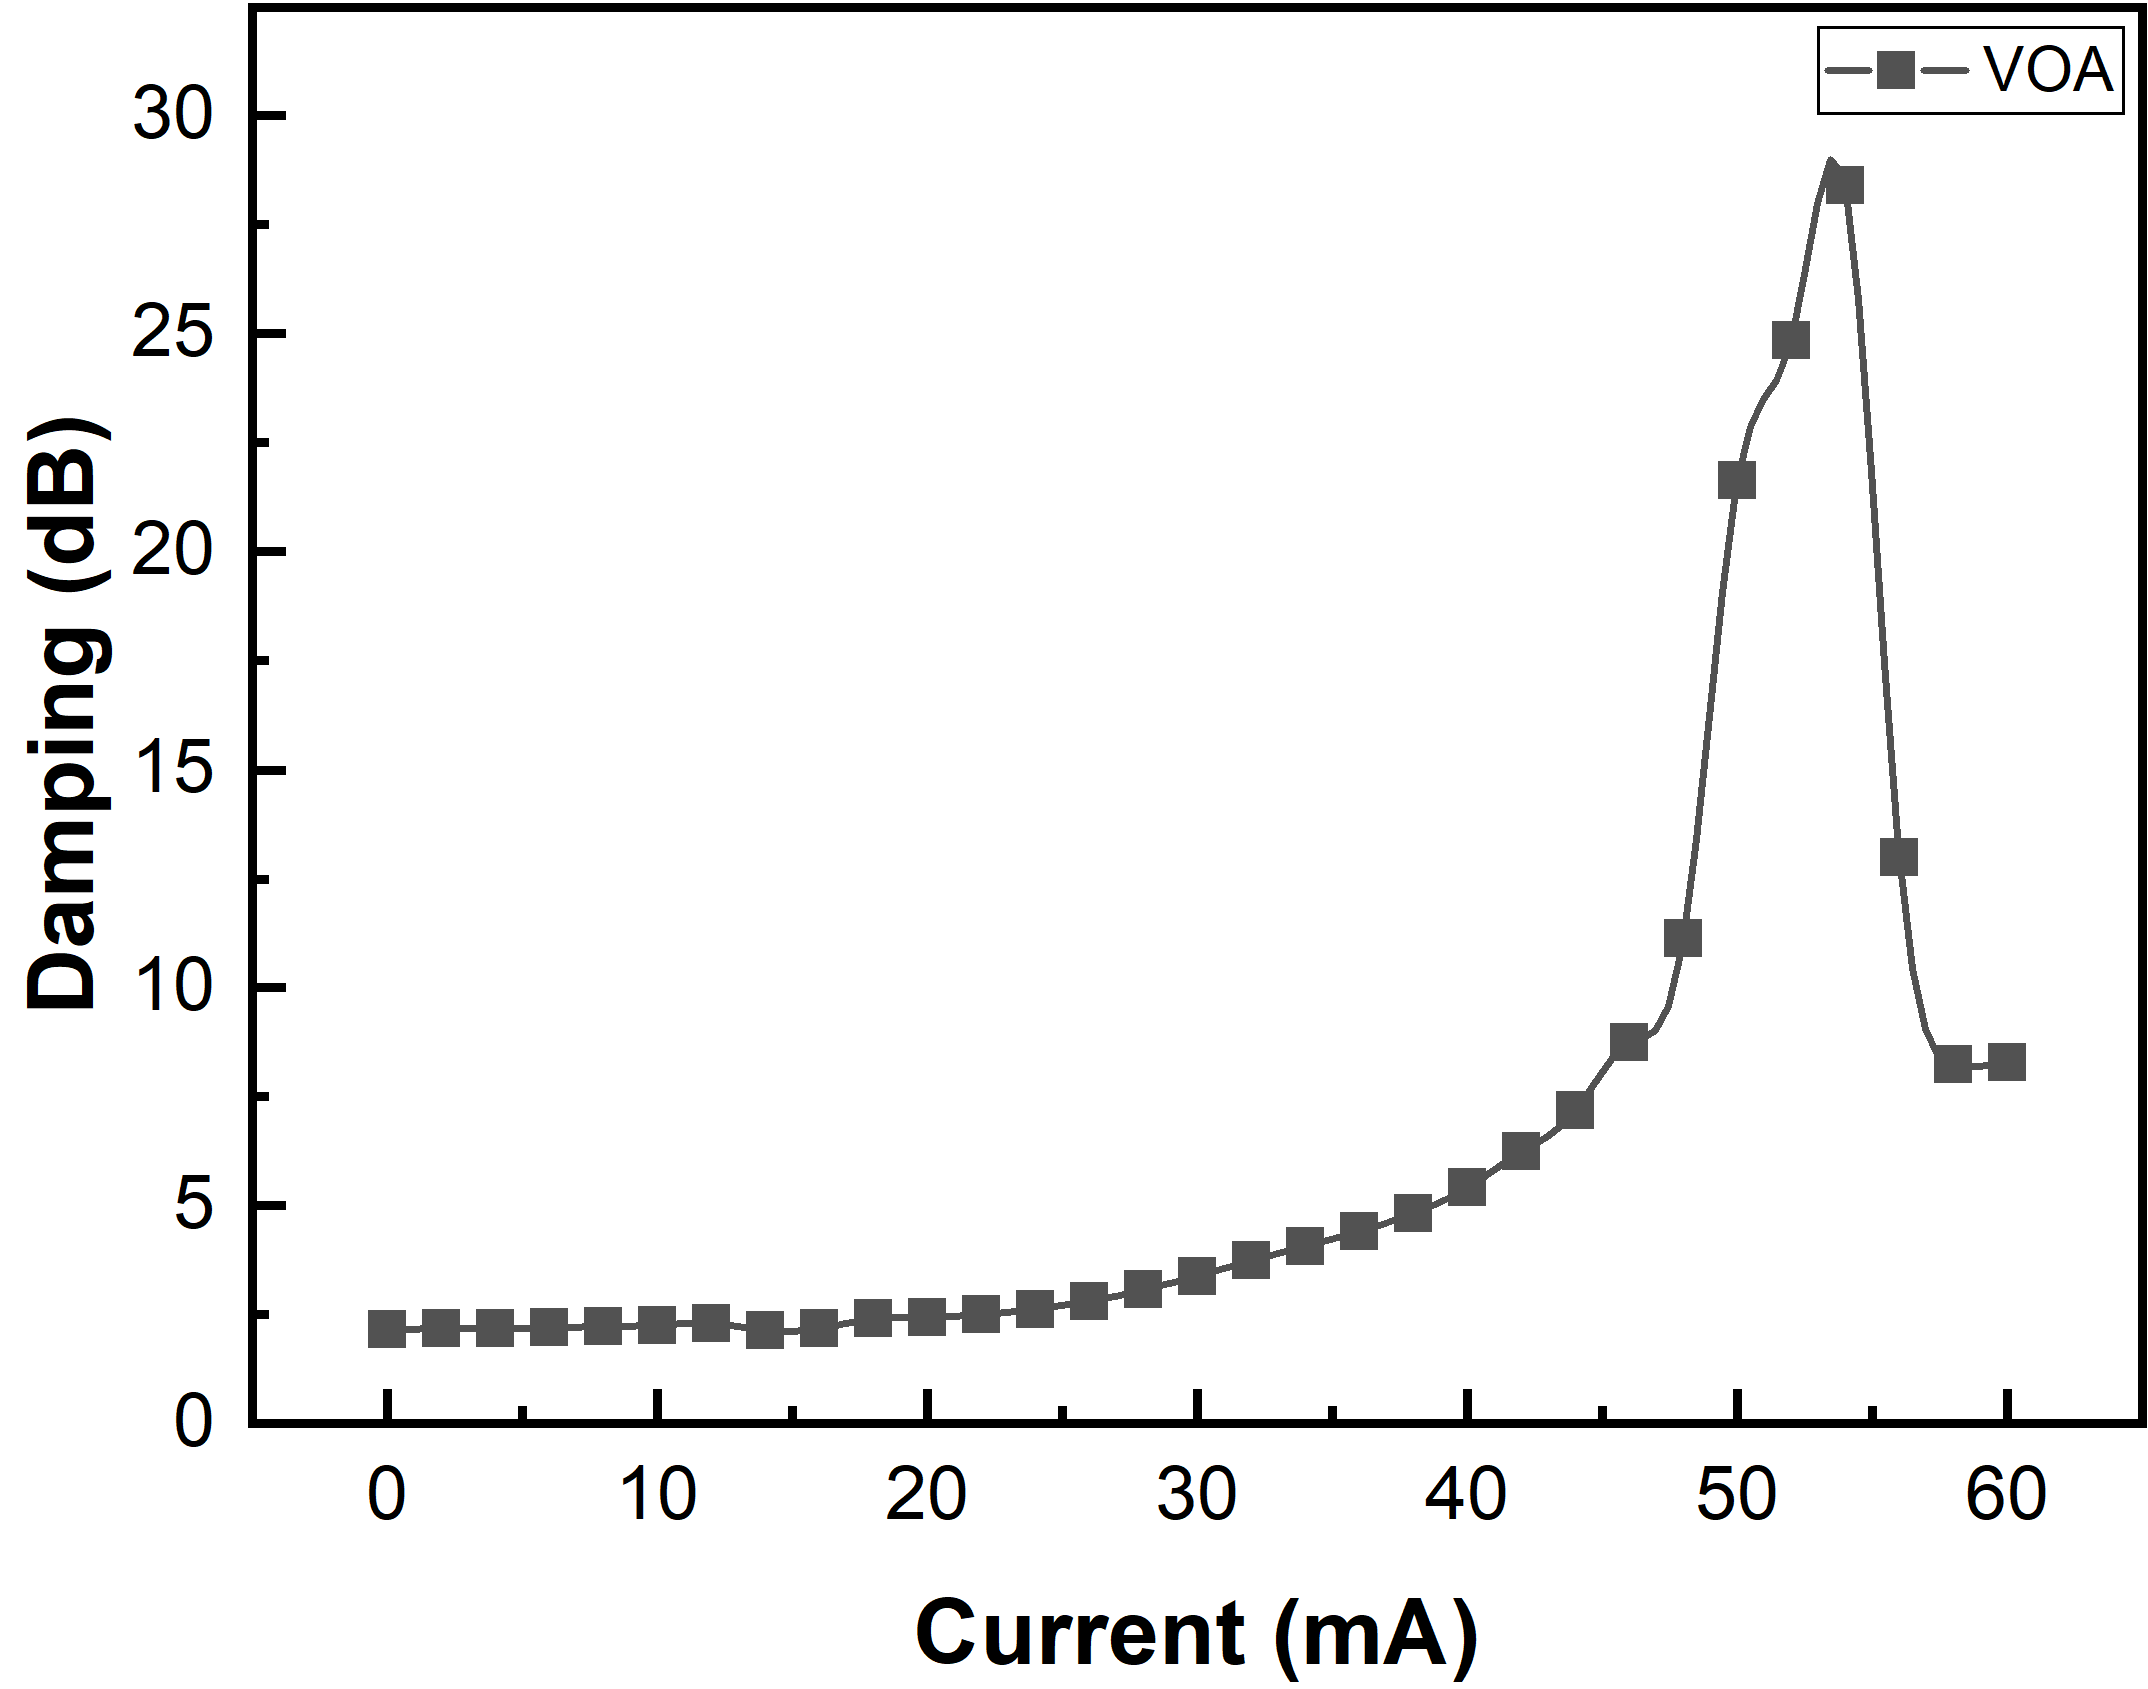
\includegraphics[width=0.6\linewidth]{figures/VOA_18321.png}
    \caption{Characterization of the VOA with maximum $-28.39 \ dB$ damping achieved at current value of $54 \ mA$.}
    \label{fig:VOA_18321}
\end{figure}

\subsubsection{Observed Photon-Photon Resonance} \label{subsubsec:observed_PPR}
Bandwidth enhancement by PPR is achieved with this short external feedback design. As shown in \autoref{fig:spectra_and_bandwidth_6559}, the appearing of the second resonance peak in the frequency response is clearly different from the ones presented in \autoref{fig:undamped_RO_measurement}. The mode spacing of $15.2 \ GHz$ is correspoing to the external feedback section design of $4869.76 \ \mu m$ with FSR of $15.9 \ GHz$, the appearing of PPR with value of $14.8 \ GHz$ is slightly lower than the FSR value but in the same order. By tuning the phase section in the external feedback section, the side mode shifts to the main mode and the PPR mode also moves toward the first peak which is CPR. Further tuning the phase section with the mode spacing close to the self mode locking range, the undamped RO starts to dominate and finally breaks the stable lasing condition.

\begin{figure}[H]
    \centering
    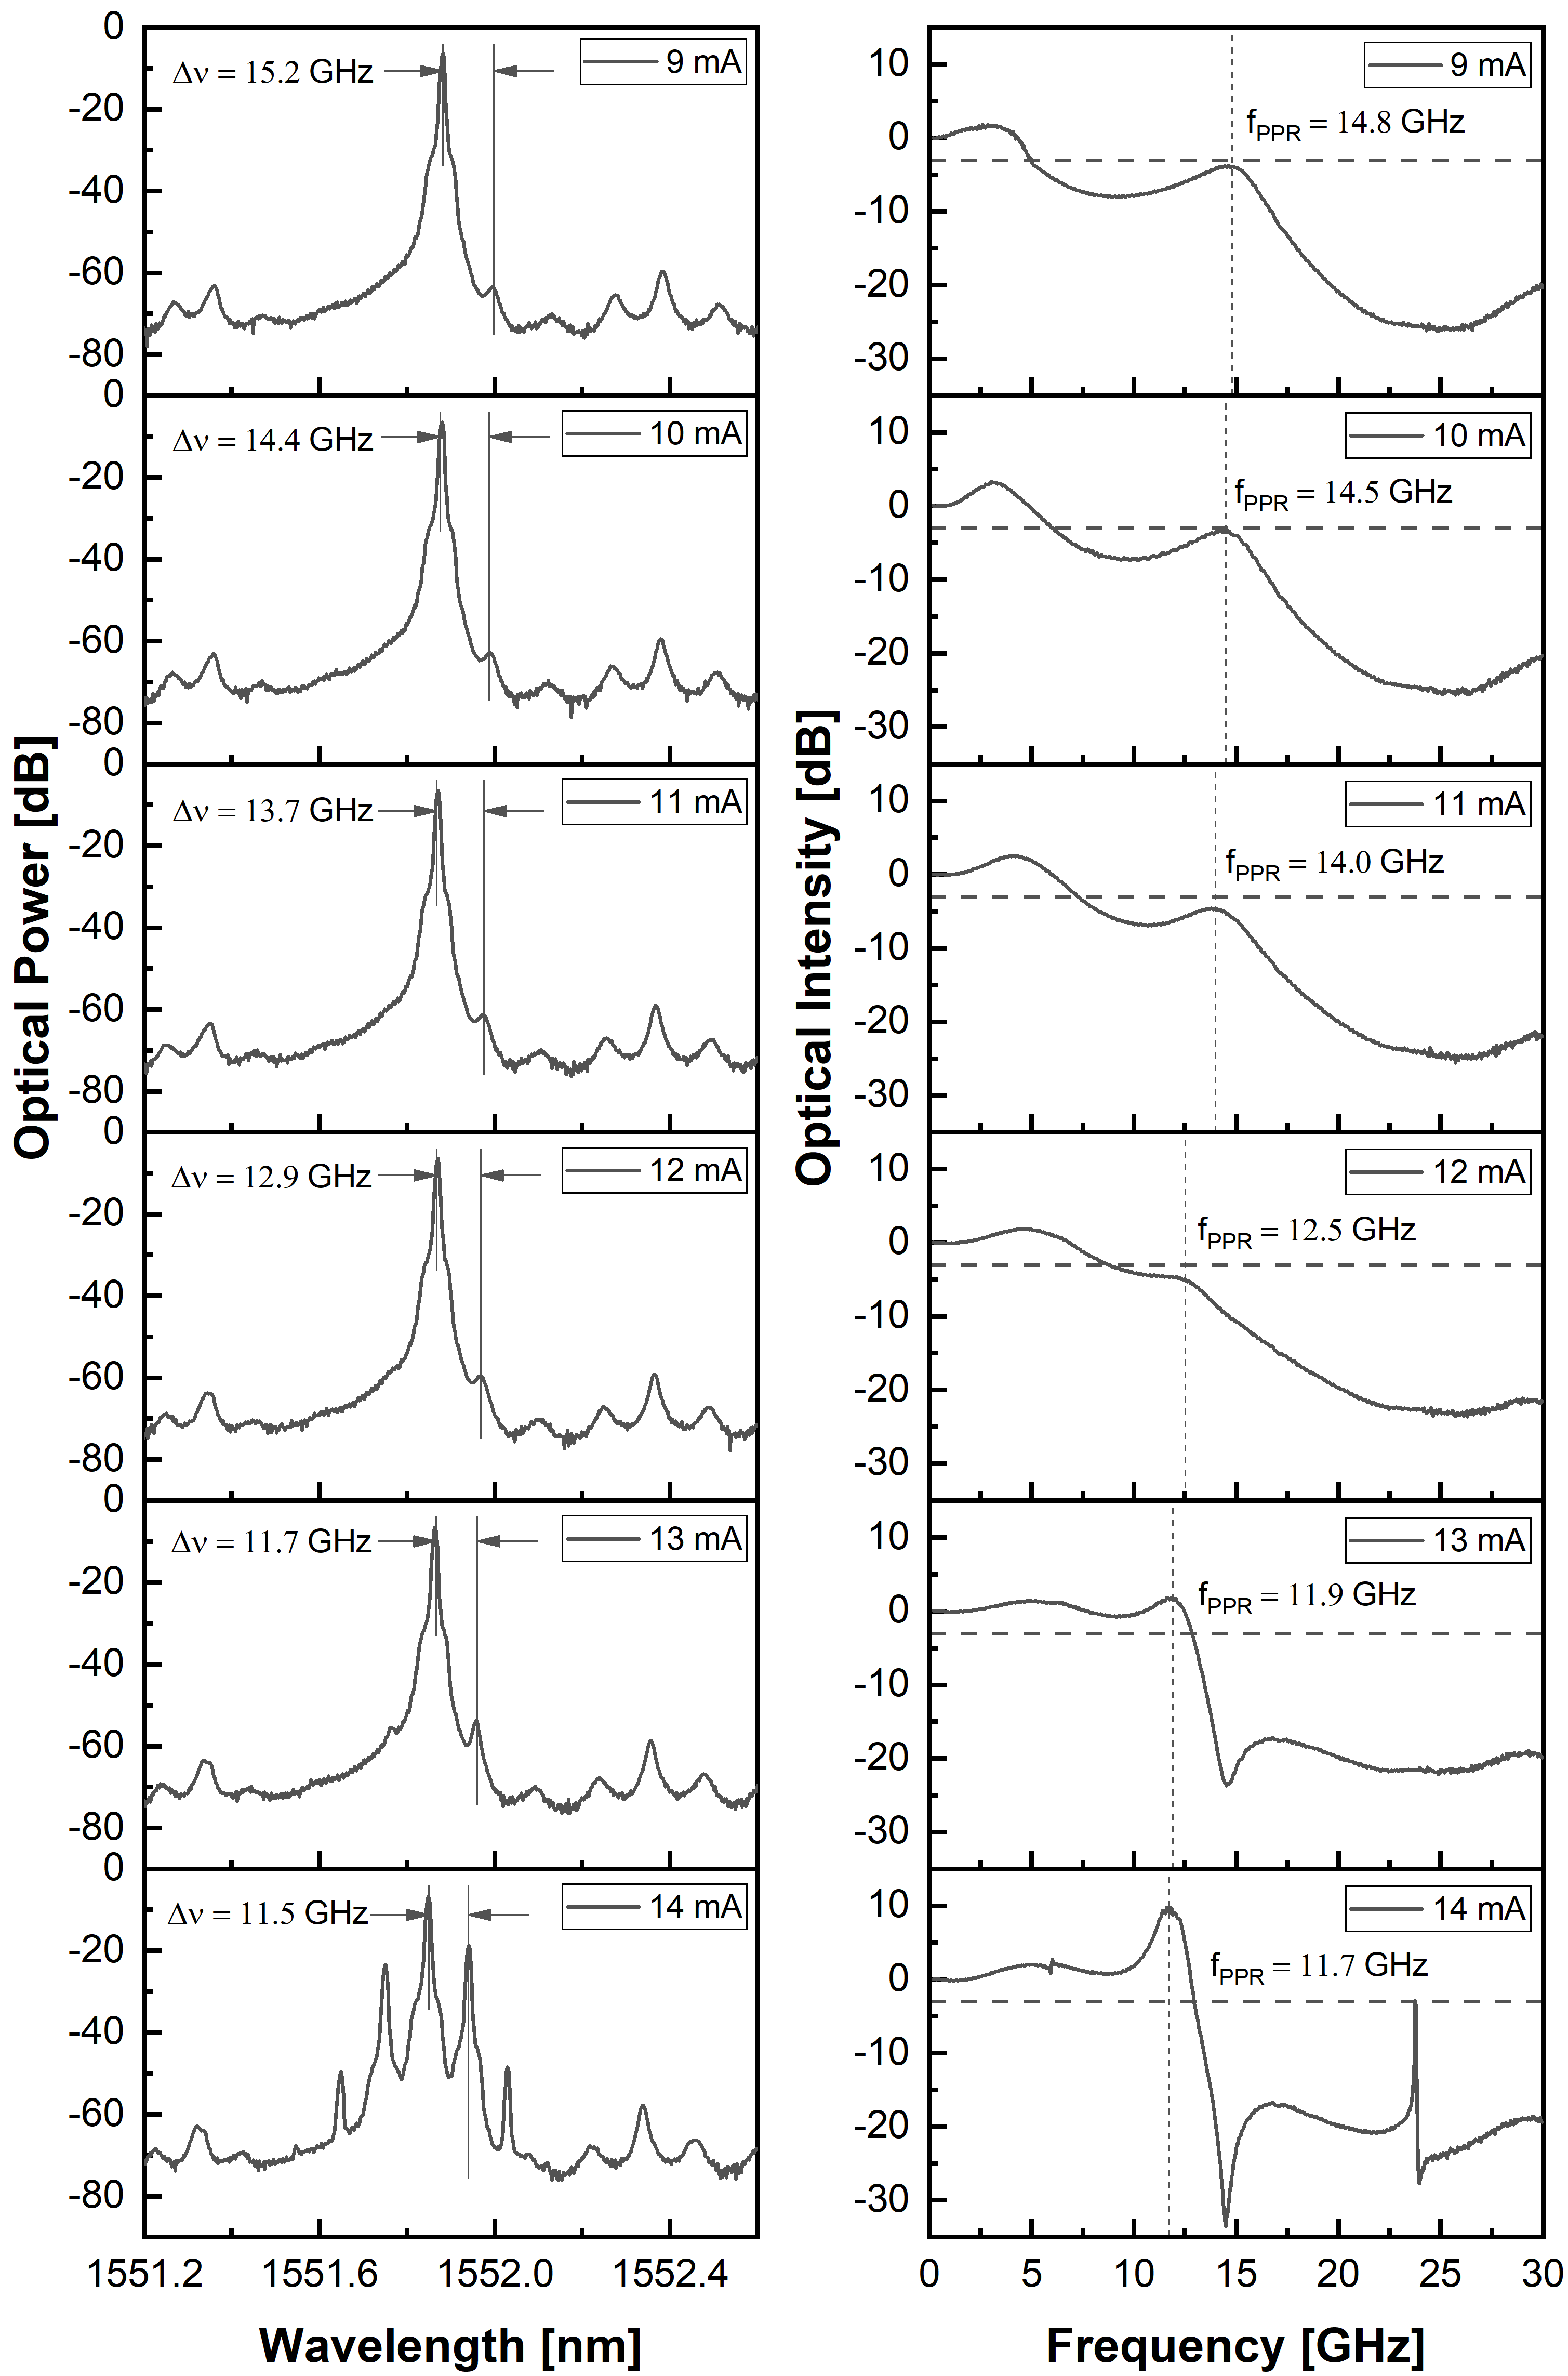
\includegraphics[width=.9\linewidth]{figures/spectra_and_bandwidth_6559.png}
    \caption{Spectra and frequency response of the short external feedback device. Moving of the side peak in spectra and shifting of the second resonance peak in frequency response is observed by shifting the external feedback phase current.}
    \label{fig:spectra_and_bandwidth_6559}
\end{figure}

The best achieved bandwidth value of $f_{3dB}=13.2 \ GHz$ with PPR is shown in \autoref{fig:spectra_and_bandwidth_6557}, with the external cavity length of $6359.76 \ \mu m$ and the designed FSR of $12.9 \ GHz$. The mode spacing between the main mode and the side mode is $11.5 \ GHz$ and the PPR is appearing at $11.6 \ GHz$ in the frequency response.

\begin{figure}[ht]
    \centering
    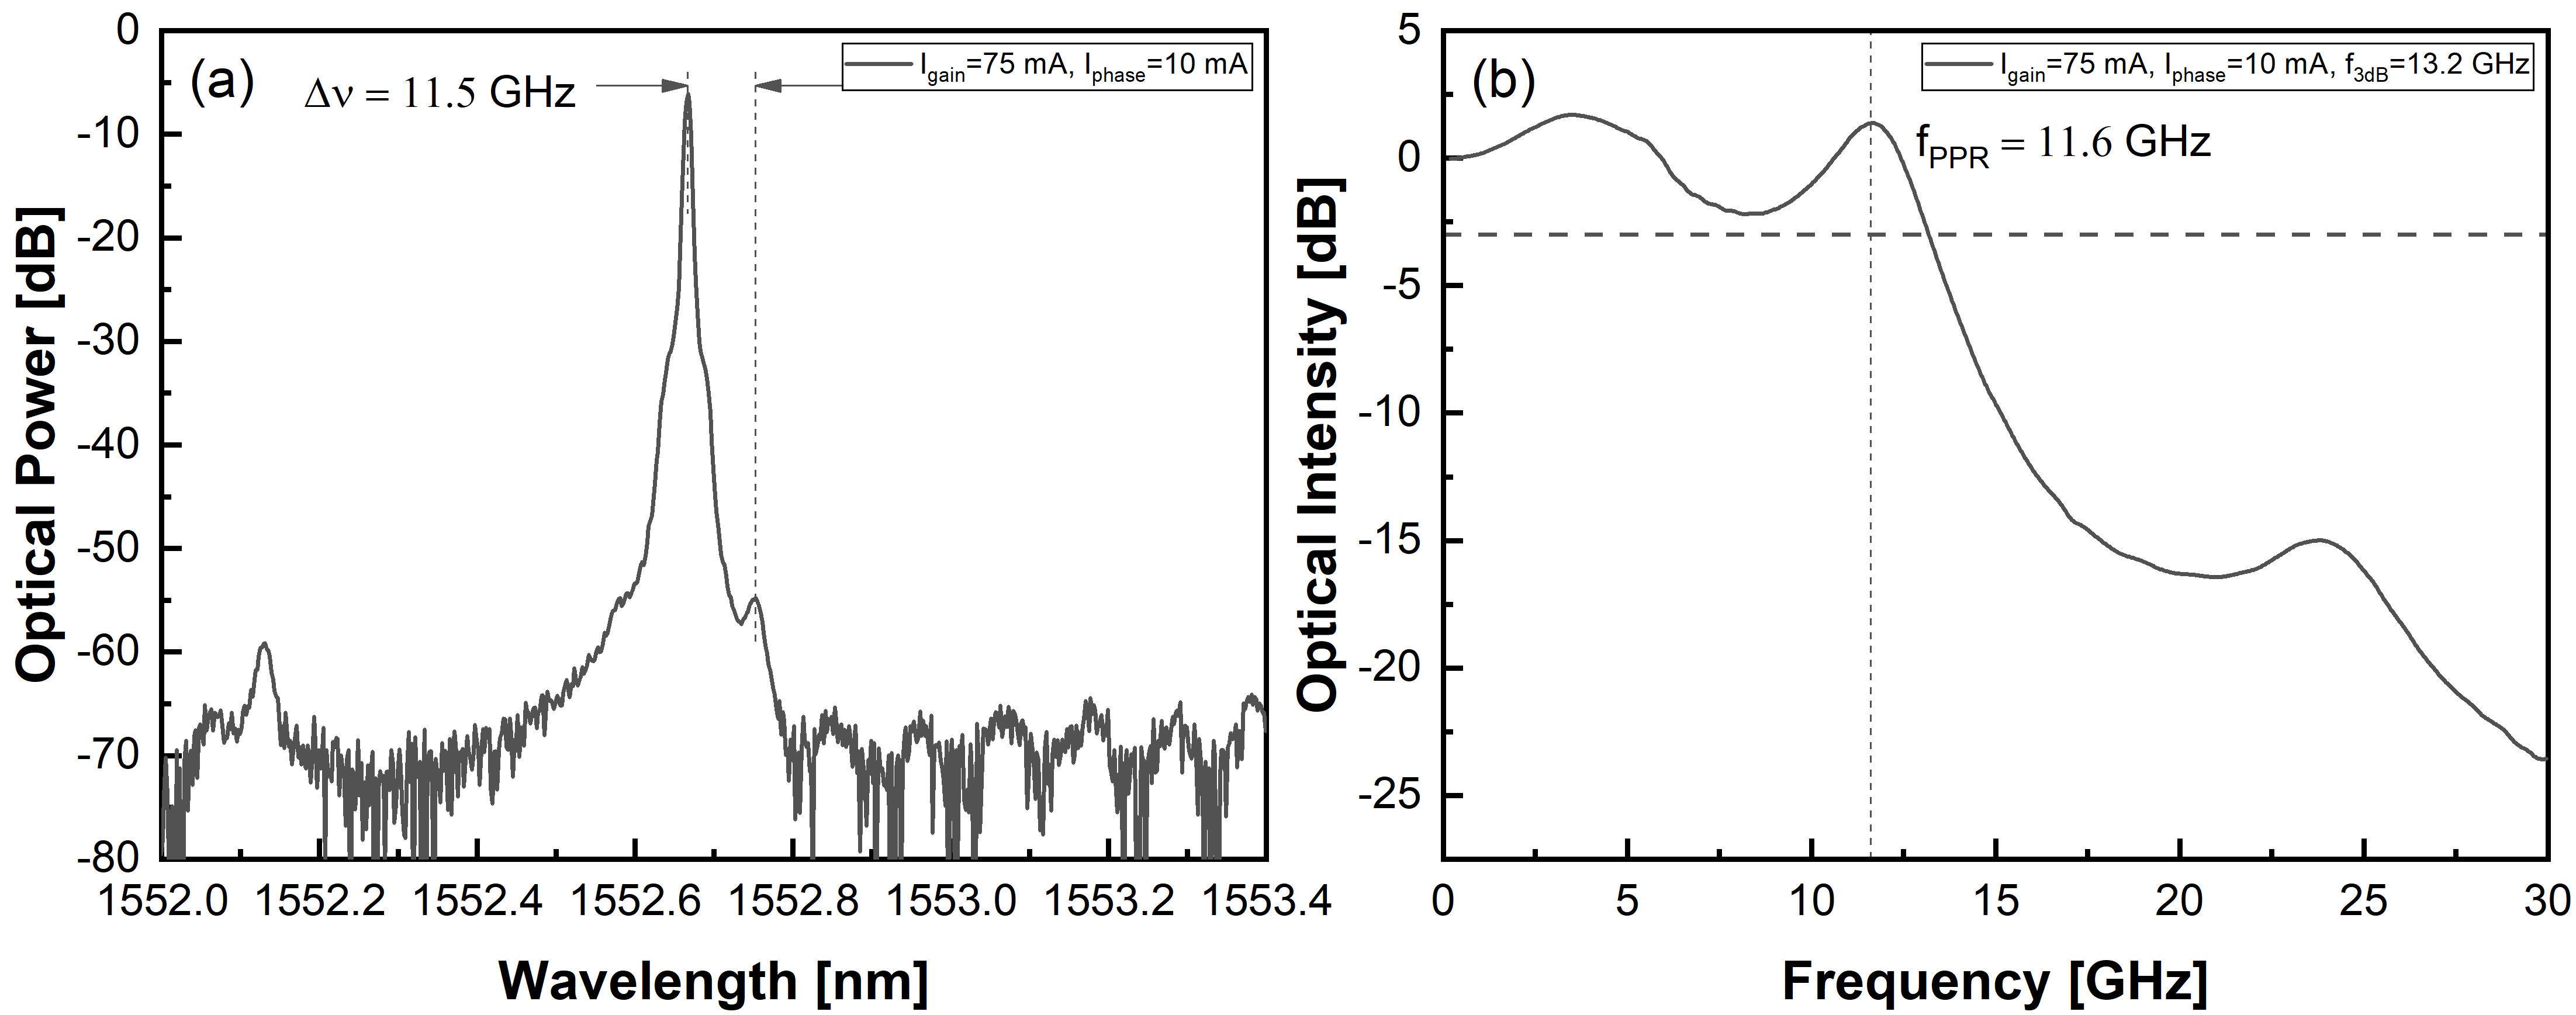
\includegraphics[width=\linewidth]{figures/spectrum_and_bandwidth_6557.png}
    \caption{The best achieved bandwidth value of $f_{3dB}=13.2 \ GHz$ with PPR. The external cavity length is $6359.76 \ \mu m$ corresponds to the FSR value of $12.9 \ GHz$. The mode spacing between the main mode and the side mode is $11.5 \ GHz$ and the PPR is appearing at $11.6 \ GHz$ in the frequency response.}
    \label{fig:spectra_and_bandwidth_6557}
\end{figure}

Chirp reduction is also observed by tuning the phase in the external feedback section, the result is shown in \autoref{fig:chirp_6559} and \autoref{tab:chirp_6559}. Tuning the phase current from $10 \ mA$ to $14 \ mA$ allows the increase of the $\alpha$ parameter from $1.793$ to $3.245$. Note that the current value in \autoref{tab:chirp_6559} is $1 \ mA$ higher than the value in \autoref{fig:spectra_and_bandwidth_6559} because of the existance of the hysteresis.

\begin{figure}[H]
    \centering
    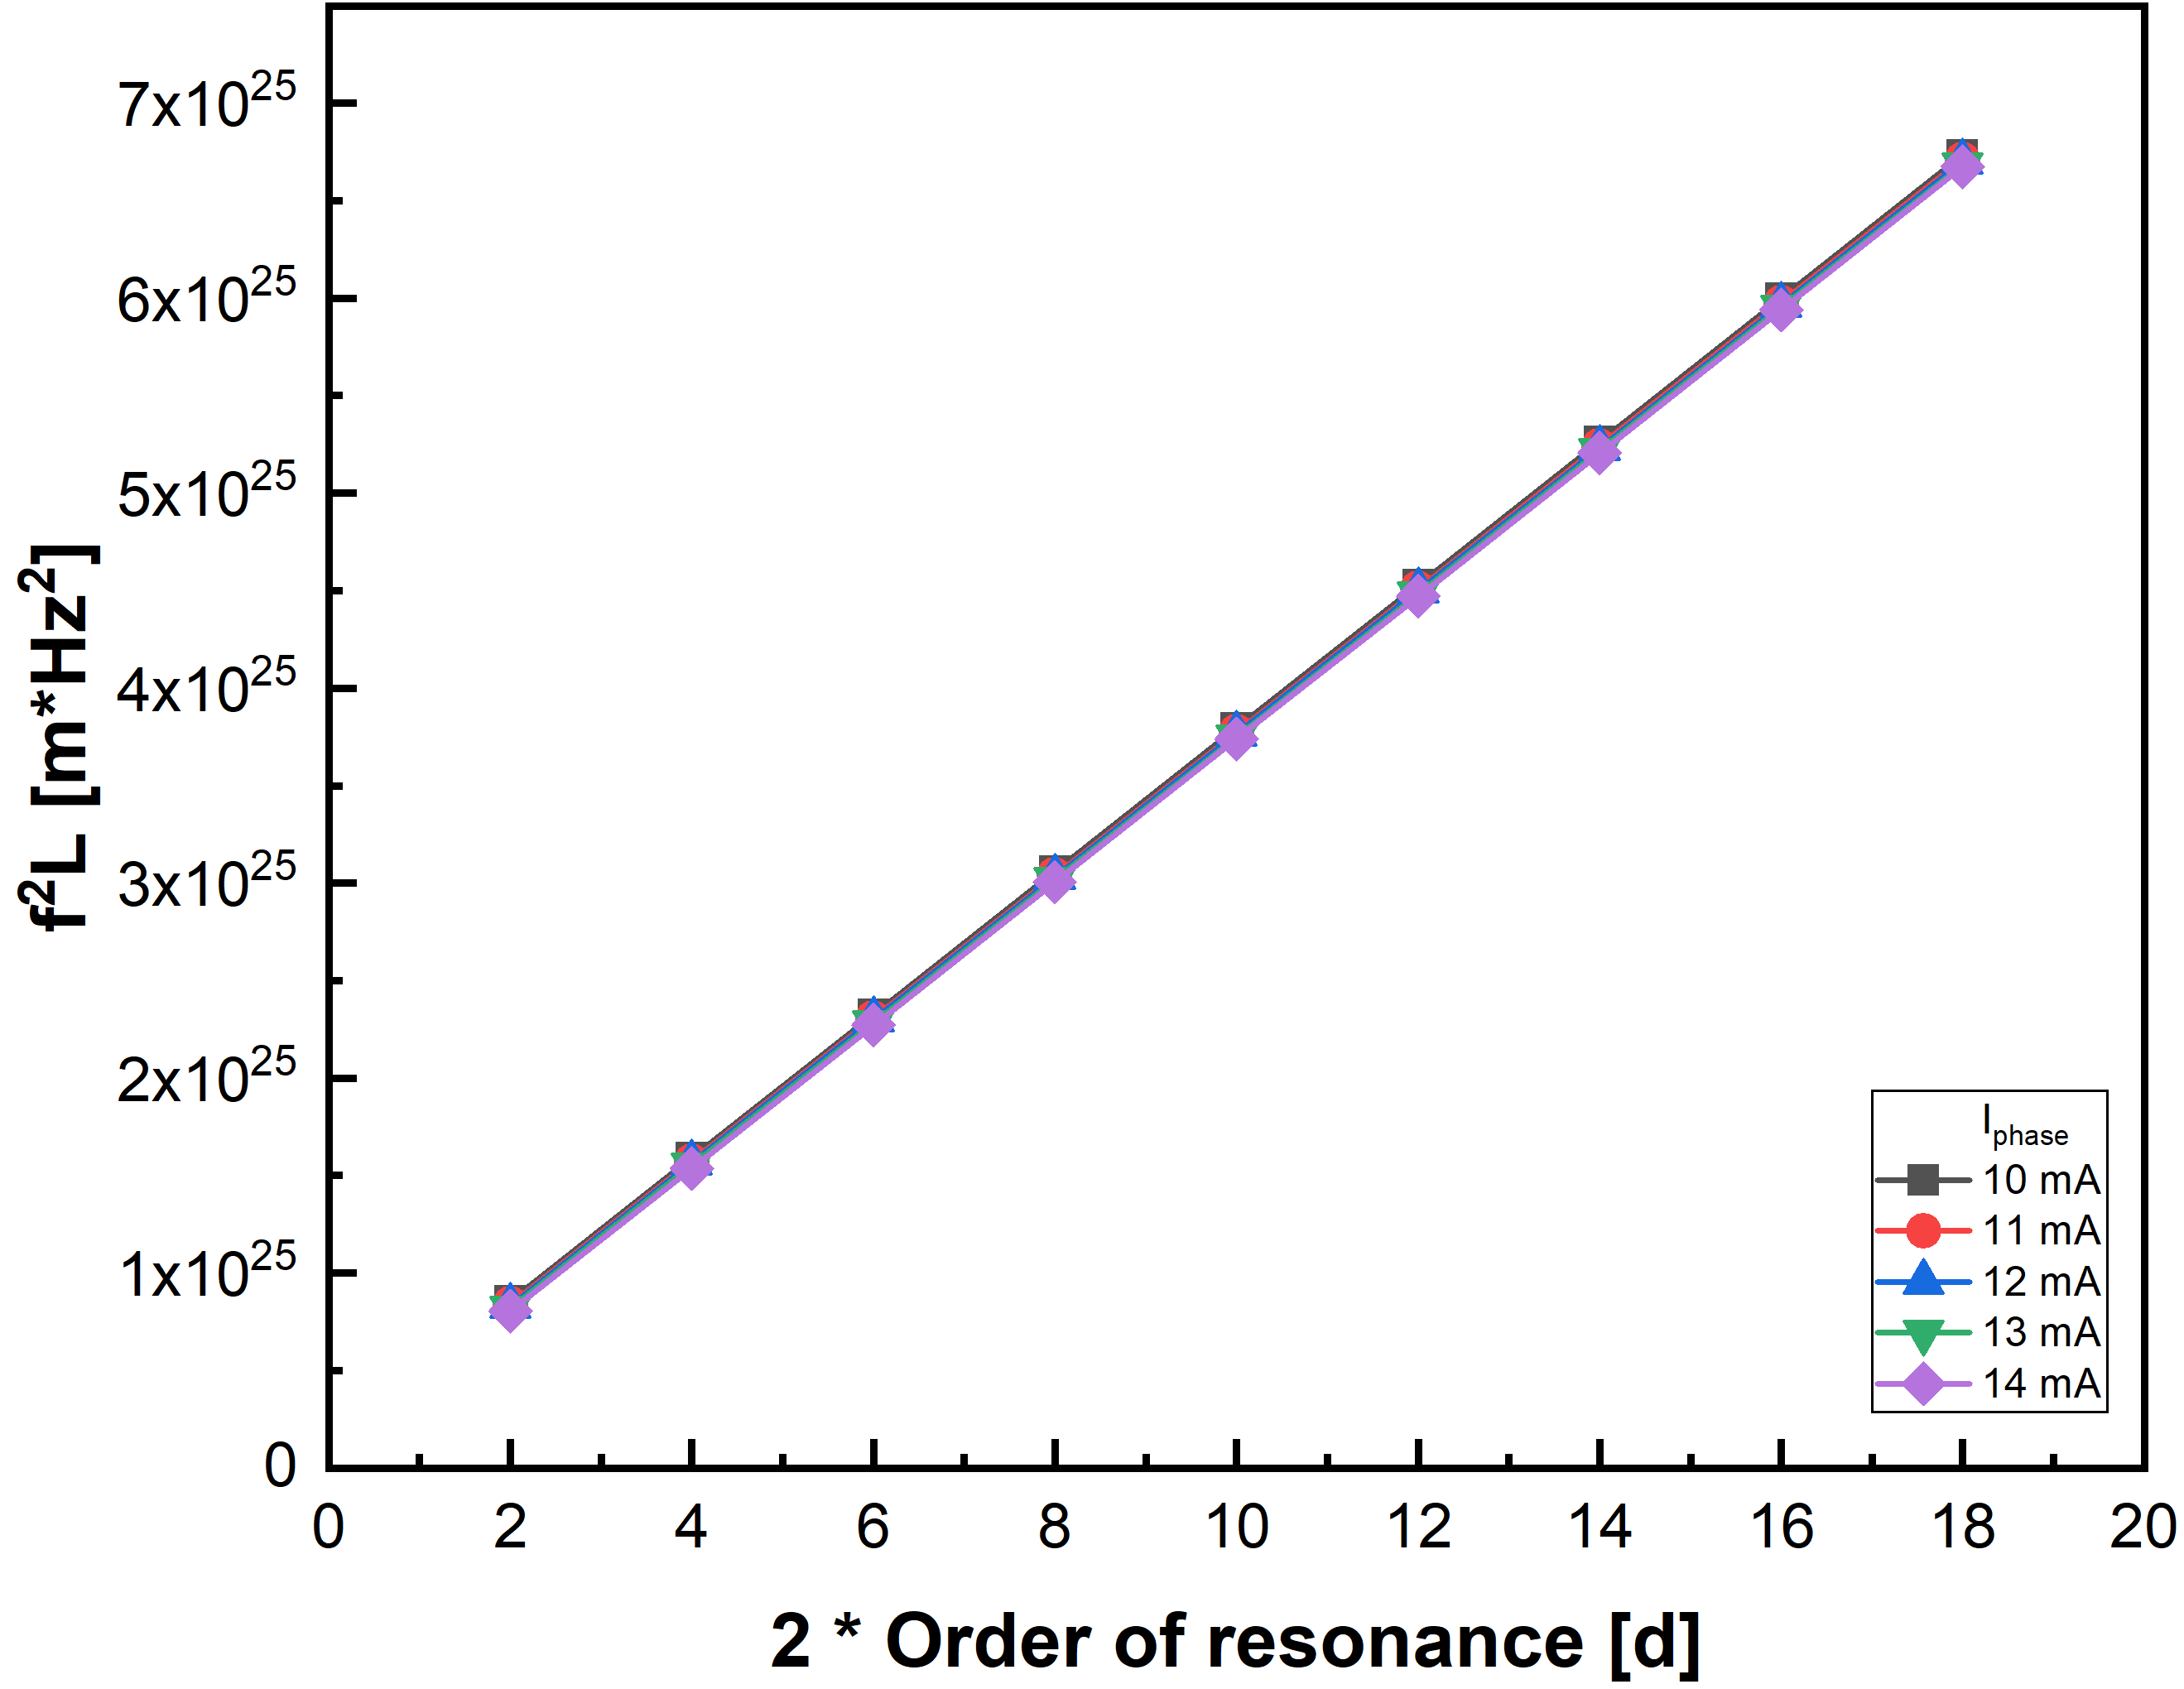
\includegraphics[width=.7\linewidth]{figures/chirp_6559.png}
    \caption{Linear regression fit for phase current from $10 \ mA$ to $14 \ mA$.}
    \label{fig:chirp_6559}
\end{figure}

\begin{table}[ht]
    \centering
    \caption{Measured chirp parameter $\alpha$ by fixing the gain current at $75 \ mA$ and scan the phase section in the external feedback section from $10 \ mA$ to $14 \ mA$. Increasement of the chirp parameter $\alpha$ is observed from $1.793$ to $3.245$}.
    \label{tab:chirp_6559}
    \resizebox{\textwidth}{!}{%
    \begin{tabular}{@{}llllll@{}}
    \toprule
    \multirow{2}{*}{$I_{gain} \ [mA]$} & \multicolumn{5}{c}{$\alpha$}                                                                                \\ \cmidrule(l){2-6} 
                                      & $I_{phase}=10 \ mA$ & $I_{phase}=11 \ mA$ & $I_{phase}=12 \ mA$ & $I_{phase}=13 \ mA$ & $I_{phase}=14 \ mA$ \\ \midrule
    75                                & 1.725               & 2.063               & 2.220               & 2.624               & 3.247               \\
    75                                & 1.818               & 1.991               & 2.296               & 2.618               & 3.257               \\
    75                                & 1.818               & 2.070               & 2.246               & 2.614               & 3.253               \\
    75                                & 1.808               & 2.054               & 2.242               & 2.566               & 3.221               \\ \midrule
    Average                           & 1.793             & 2.045              & 2.251               & 2.606              & 3.245              \\ \bottomrule
    \end{tabular}%
    }
\end{table}

The reason for the change of the $\alpha$ with respect to change of the phase current may relates to the slope of the feedback altered grating response as discussed in \autoref{subsec:feedback_introduced_detuned_loading}. By changing the phase current it shifts the lasing mode along the RTG curve towards the central peak which decreases the slope and in turn decreases the $B$ parameter.

\subsection{Long Feedback Cavity} \label{subsec:long_feedback_cavity}
Follows the same design principle as in \autoref{subsec:short_feedback_cavity}, the long feedback section is achieved by the spiral structure with the circle bending radius of $1500 \ \mu m$. The on-chip long feedback design is shown in \autoref{fig:grating_5742_design}. The spiral structure has a variable design to achieve external cavity length of [39.28, 55.70, 81.33, 86.53, 100.75, 157.35] $\ mm$ by using \autoref{eq:F_weak_feedback} and \autoref{eq:F_strong_feedback}.

\begin{figure}[H]
    \centering
    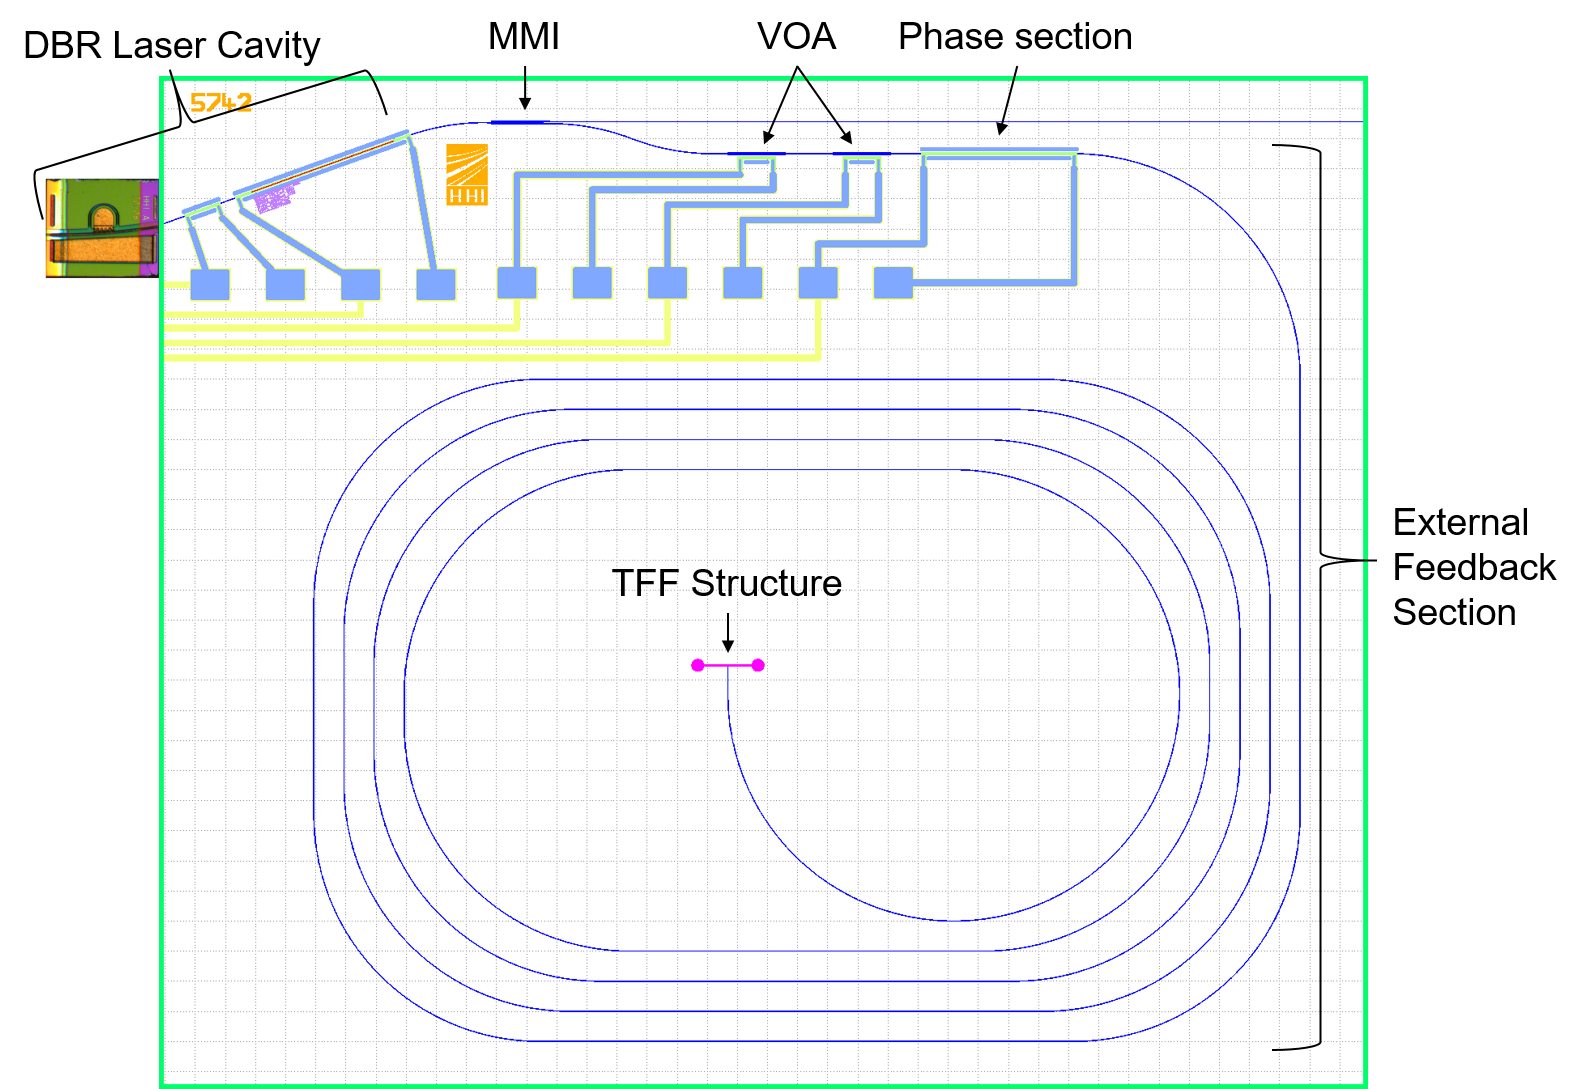
\includegraphics[width=0.8\linewidth]{figures/5742_spiral_comment.png}
    \caption{Chip design of the laser with a long external section and controllable feedback.}
    \label{fig:grating_5742_design}
\end{figure}

The example of produced photonic integrated circuits (PICs) and grating characterization is shown in \autoref{fig:grating_5742}. Similliar ripples were observed in the reflection curves but not in the transmission curves, it may because the attenuation inside the polymer waveguide after the spiral structure is relative high so that the reflected from the TFF slot got attenuated.

\begin{figure}[ht]
    \centering
    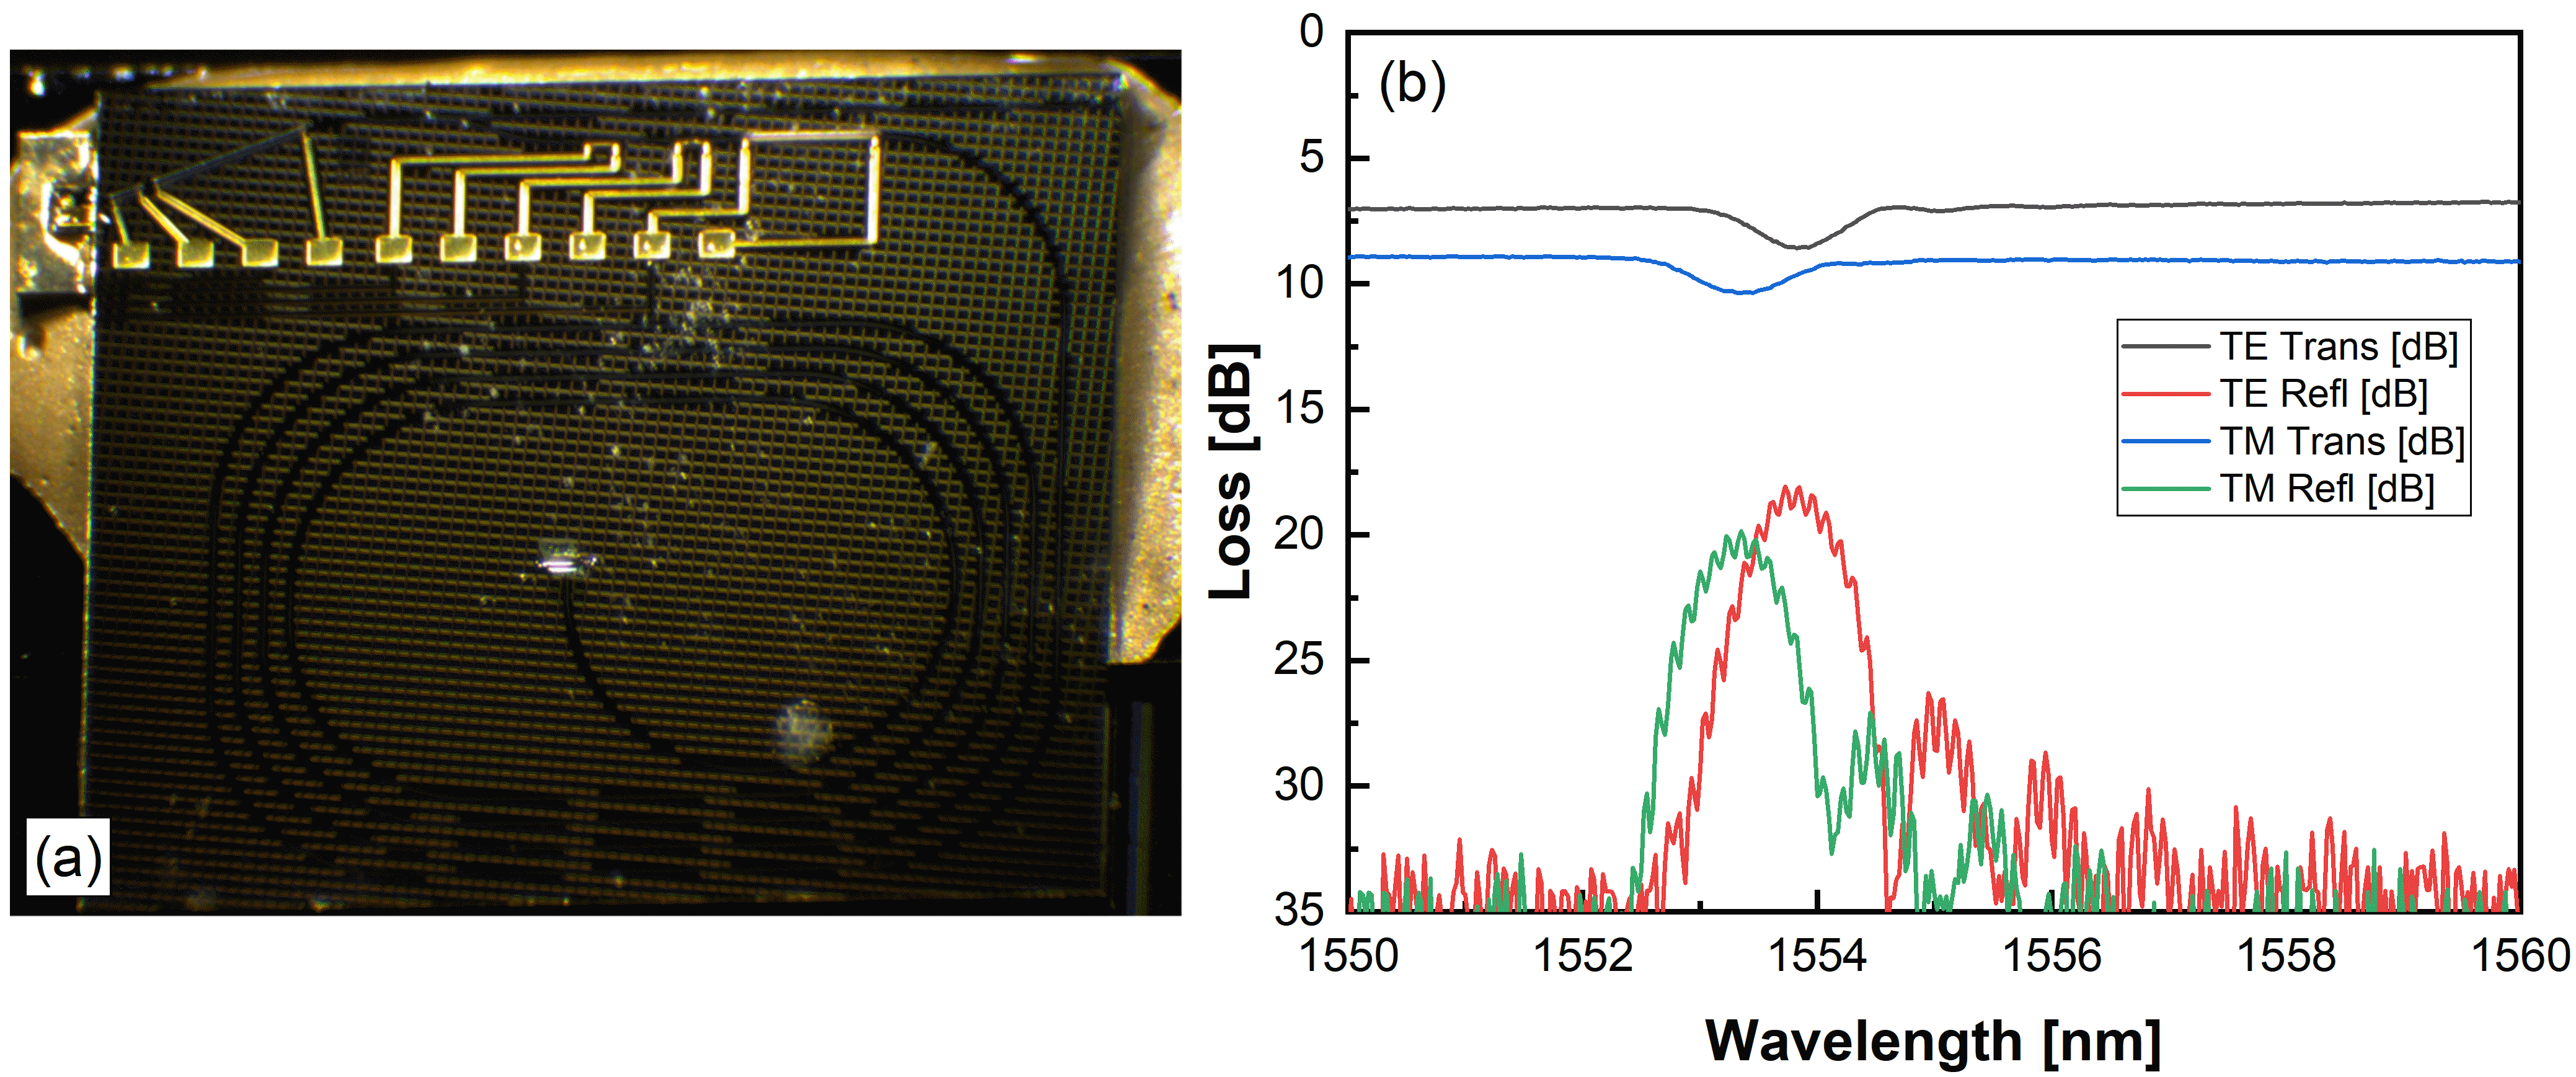
\includegraphics[width=\linewidth]{figures/grating_5742.png}
    \caption{(a) Produced photonic integrated circuits (PICs) with long feedback design, (b) grating characterization of the device, the spacing of the ripples in the reflection (red and green) curves are corresponding to the distance between MMI and output port.}
    \label{fig:grating_5742}
\end{figure}

Linewidth was measured using the same principle as in \autoref{sec:linewidth_measurement}. External feedback phase curent $I_{ext_{phase}}$ was shifted from $14 \ mA$ to $30 \ mA$ with the step of $0.2 \ mA$ and the possible phase dependent linewidth reduction can be seen in \autoref{fig:linewidth_and_spectra_5742}. 
% The maximum achieved linewidth is $0.857 \ MHz$ and the minimum is $0.186 \ MHz$.

\begin{figure}[ht]
    \centering
    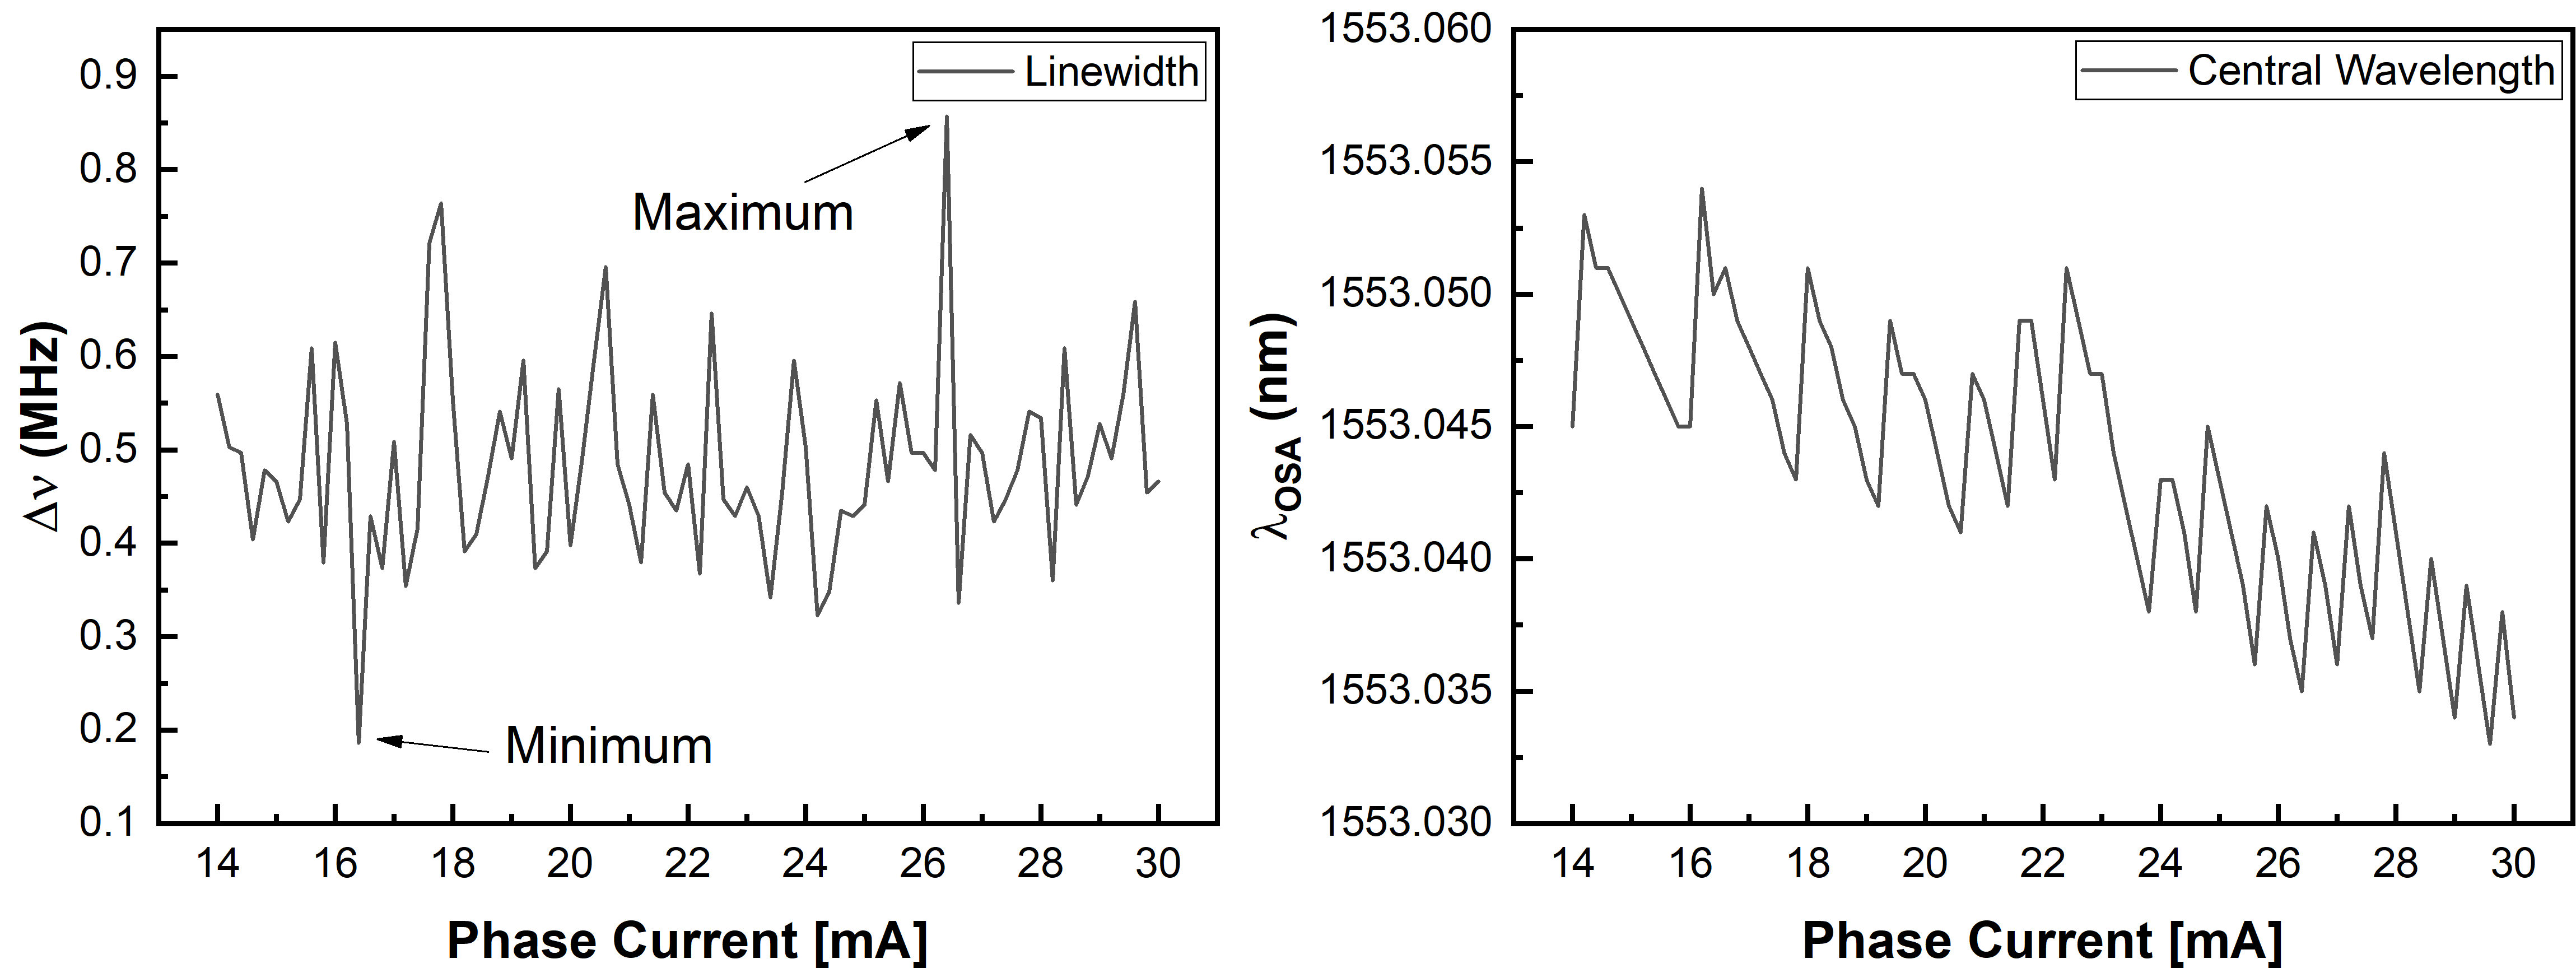
\includegraphics[width=\linewidth]{figures/linewidth_and_spectra_5742.png}
    \caption{}
    \label{fig:linewidth_and_spectra_5742}
\end{figure}

% \begin{table}[ht]
%     \centering
%     \caption{My caption}
%     \label{my-label}
%     \begin{tabular}{@{}lll@{}}
%     \toprule
%                         & Maximum & Minimum \\ \midrule
%     $\Delta\nu \ [MHz]$ & 0.857   & 0.186   \\ \bottomrule
%     \end{tabular}
% \end{table}

Since from the grating characterization a possible high attenuation in the waveguide is observed, which leads to a assumption that this device is operating under relative weak feedback with paramter $C<1$. From the wavelength scan a periodic shifting of the central wavelength indicates the feedback introduces a periodic effect to the laser cavity. With \autoref{eq:F_weak_feedback}, the periodic behavior was modeled with $\cos(\phi_{ext}+\arctan\alpha)$ term with the feedback round trip phase $\phi_{ext}$ included. More characterization needs to be done on such device since the minimum value achieved in \autoref{fig:linewidth_and_spectra_5742} is one isolated point in the scan of the phase, which could be not correctly calculated.



% The parameter $F$ strongly depends on the phase of the externally reflected light $\phi_{ext}$ a very careful control of $\phi_{ext}$ is required for achieving a certain linewidth narrowing
